\newpage
\section{Approach}
\label{sec:Approach}
In the following the methods developed within the underlying project are
presented. After introducing into the general design of \ac{TAD} in
\mysecref{sec:Approach_GD} the implementation for each task are shown, i.e. for
\ac{SISR} in \mysecref{sec:Approach_ID}, for \ac{VSR} in
\mysecref{sec:Approach_VD} and for \ac{IC} in \mysecref{sec:Approach_IC}.

\subsection{General Design}
\label{sec:Approach_GD}
The general idea behind \ac{TAD} is that a high-dimensional input (e.g. a
high-resoluted or colored image) is transformed in a low-dimensional space so
that it first can be inverse transfored as good as possible and second still is
human-understandable in lower dimensional space. Besides, both transformations
should be computationally efficient.

\subsubsection*{Autoencoder Network Design}
In order to fulfill the requirements above an reasonably shallow autoencoder is
used, consisting of a combination between convolutional and subpixel convolutional
(pixel-shuffle and inverse pixel-shuffle) layers, as shown in
\myfigref{fig:architecture} using the example of \ac{SISR}.
\newline
In the first part, $g_\phi$, a high-dimensional input (left: \ac{HR}) is first
filtered using two convolutional layers, then downscaled using inverse subpixel
convolutions. Afterwards several \textit{Resblocks} perform further
transformations, followed by two convolutional layers. As discussed below the
encoding is added to a trivially interpolated low-dimensional representation
(lower middle: \ac{LR}) forming the autoencoder's \ac{SLR} (upper middle).
The inverse transformation, $f_\theta$, has a similar inversed structure and
results in the \ac{SHR} (right).

\begin{figure}[!htbp]
	\centering
	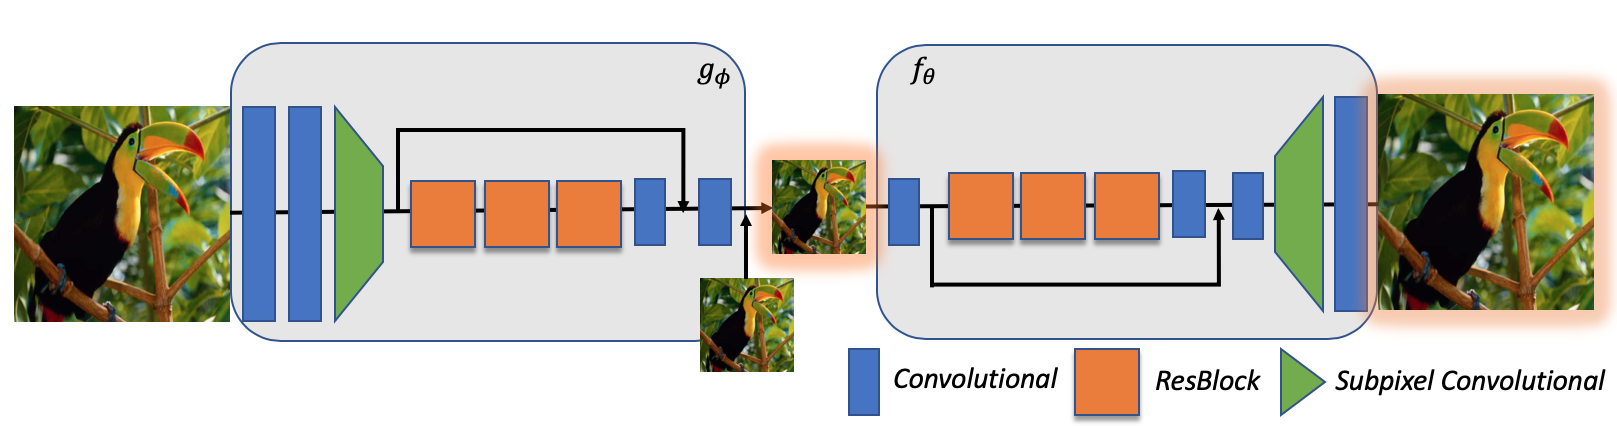
\includegraphics[width=12cm]{figures/architecture}
	\caption{Overview of \ac{TAD} autoencoder network design for \ac{SISR} task.}
  \label{fig:architecture}
\end{figure}

Thereby, a \textit{Resblock} is a convolutional-recurrent sequence as follows:

$$Resblock(x) = x + Conv2D(ReLU(Conv2D(x)))$$

The \textit{Resblocks} are important to conserve information throughout the
layers, as demonstrated in \mychapterref{sec:ExperimentsandResults} the number of
\textit{Resblock} has a large impact on both the performance and runtime of the
model.
\newline
Since this network design does not continuously downscales the input but
applies inverse pixel shuffeling to downscale while all other layers of the
downscaling network $g_\phi$ do not alter their inputs shape (and vice versa
for the upscaling network $f_\theta$), the networks can be easily modified.
\newline
The overall network structure is similiar (although not identical) to the
network purposed in \cite{TAID}.

\subsubsection*{Loss Function}
The loss function $L$ consists of two parts: The first one, $L_{TASK}$, is
task-dependent and states the difference between the decoders output $X_{SHR}$
and the desired output $X_{GT}$, e.g. the original \ac{HR} in the \ac{SISR} task.

$$L_{TASK} = L1(X_{GT}, X_{SHR})$$

The second part, $L_{LATENT}$, encodes the human-readibility of the low-dimensional
representation. To do so it is assumed that the optimal latent space encoding
is not equal but similar to trivial lower dimensional representation like a
(bilinear) interpolated \ac{LR}. Next to simplifying the loss function this
assumptions has the benefit of ensuring (faster) convergence, since merely a
difference between the interpolated representation and the more optimal encoding
has the be derived in the learning process. Also the down- and upscaling can be
learnt more \textit{independently} since the lower dimensional representation
is always guaranteed to be \textit{useful} for upscaling. So $L_{LATENT}$ is the
distance between the interpolated guidance image $X_{GD}$ and the
actual encoding $X_{SLR}$:

$$L_{LATENT} = \begin{cases}
L1(X_{GD}, X_{SLR}) & \text{if } ||L1/d_{max}|| \geq \epsilon
\\ 0.0 & \text{otherwise}
\end{cases}$$

with $||L1/d_{max}||$ being the $L1(X_{GD}, X_{SLR})$ loss normalized
by the maximal deviation between $X_{GD}$ and $X_{SLR}$. Hence,
$L_{LATENT}$ is zero in an $l1$-ball around the guidance image, ensuring that
\ac{SLR} is close to the guidance image but also helps to prevent overfitting to
the trivial solution $X_{GD} = X_{SLR} \Leftrightarrow g_\phi = 0$.
\newline
The overall loss function is a weighted sum of both of the loss function
introduced above. The relative weight $(\alpha, \beta)$ is of large importance for the
trade-off between the readibility requirement and the performance of the model's
upscaling part (super resolution, colorization). However, since the readibility
requirement typically is \textit{weaker} (i.e. \textit{easier} to fulfill since
the network is guided by a well-readable low-dimensional image) typically
$\alpha >> \beta$.

$$L = \alpha L_{TASK} + \beta L_{LATENT}$$

\subsection{Task-Aware Image Downscaling}
\label{sec:Approach_ID}


\subsection{Task-Aware Video Downscaling}
\label{sec:Approach_VD}

\subsection{Task-Aware Image Colorization}
\label{sec:Approach_IC}


% The objectives of the ``Materials and Methods'' section are the following:
% \begin{itemize}
%  \item \textit{What are tools and methods you used?} Introduce the environment, in which your work has taken place - this can be a software package, a device or a system description. Make sure sufficiently detailed descriptions of the algorithms and concepts (e.g. math) you used shall be placed here.
%  \item \textit{What is your work?} Describe (perhaps in a separate section) the key component of your work, e.g. an algorithm or software framework you have developed.
% \end{itemize}
